% strona tytulowa pracy dyplomowej wersja z 23.03.2016, LS
% drobne modyfikacje RG (13.01.2020)

%\documentclass[a4paper,twoside,openright,11pt]{report}

% Uwaga do mnie, oneside

\documentclass[a4paper,oneside,openright,11pt]{book}
\usepackage{graphicx}
%
\usepackage{graphicx}
% pzydatne pakiety jezeli tytul zawiera symbole matematyczne:
%
%\usepackage{english}
\usepackage{amsmath}
\usepackage{amssymb}
\newtheorem{theorem}{Postulate}
\usepackage{listings}
\usepackage{amsfonts}
\usepackage{biblatex}
\usepackage{appendix}
\addbibresource{biblio.bib}

\usepackage[utf8]{inputenc}
\usepackage[T1]{fontenc}

\usepackage{hyperref}

\usepackage[section]{placeins}




%
%\usepackage[polish]{babel}
%Jesli uzywasz kodowania polskich znakow ISO-8859-2 nastepna linia powinna byc 
%odkomentowana
%\usepackage[latin2]{inputenc}
%Jesli uzywasz kodowania polskich znakow CP-1250 to ta linia powinna byc 
%odkomentowana
%\usepackage[cp1250]{inputenc}
%
% jezeli uzywasz utf8 siegnij do dokumentacji LaTeXa
%%%%%%%%%%%%%%%%%%%%%%%%%%%%%%%%%%%%%%%%%%%%%%%%%%%%%%%%%%%%%%%%%%%%%%%%%%%%%%%%%%%%%%%%
% parametry strony, troche "na wyrost", pod katem projektu ewentualnej klasy dokumentu
\textwidth\paperwidth
\advance\textwidth -55mm
\oddsidemargin-1in
\advance\oddsidemargin 30mm
\evensidemargin-1in
\advance\evensidemargin 25mm
\topmargin -1in
\advance\topmargin 2cm
\setlength\textheight{48\baselineskip}
\addtolength\textheight{\topskip}
\marginparwidth15mm
%
% definicja strony tytulowej
% LOGO PK i WIMiF umieszczamy w tym samym katalogu co dokument
%
\renewcommand\maketitle{%
	\begin{titlepage}%
		\noindent
		\begin{minipage}[b]{0.9in}%
			
\includegraphics[width=2.2truecm]{PK_logo.png}
		\end{minipage}
		\begin{minipage}[b]{4.0in}%
			\begin{center}%
				{\LARGE\textbf{Politechnika Krakowska \\ im. Tadeusza Ko\'sciuszki}\\
					\vspace{0.2cm}
					\Large\textbf{Wydzia\l{} In\.zynierii Materia\l{}owej i Fizyki} \par}
			\end{center}
		\end{minipage}
		\begin{minipage}[b]{1in}%
			
\includegraphics[width=2.2truecm]{IMF_logo.png}
		\end{minipage}
		
		\vspace{1cm plus 1fill} 
		
		\begin{center}%
			\vspace{0.2cm}
			{\Large\bf\autor\par}
			\vspace{0.3truecm}
			{\large Nr albumu: \nralbumu\par}                                           
			\vspace{8mm plus .1fill}
			{\LARGE\textbf{\tytulpl}\par}
			\vspace{6mm}
			{\LARGE\textbf{\tytulang}\par}
			\vspace{8mm plus .1fill}
			{\large\bf Praca \rodzajpracy\\[3pt]
				kierunek: \MakeUppercase{\kierunek} \\
				specjalno\'s\'c: \MakeLowercase{\specjalnosc}
			}
			\vspace{2cm plus 1.5fill}
			\begin{flushright}\large
				\begin{tabular}{l}
					Promotor:
					\bfseries \opiekun\\ \\
					\bfseries Uzgodniona ocena:\dotfill \\[10mm]
					\dotfill\\
					podpis promotora  \qquad \qquad podpis recenzenta
				\end{tabular}
			\end{flushright}
			\vspace{1cm plus 1fill}
			{\large \textbf{\miasto\ \rok}\par}
		\end{center}
	\end{titlepage}
}
% KONIEC DEFINICJI STRONY TYTULOWEJ
%%%%%%%%%%%%%%%%%%%%%%%%%%%%%%%%%%%%%%%%%%%%%%%%%%%%%%%%%%%%%%%%%%%%%%%%%%%%%%%%%%%%%%%%%%%%%%%%%%%%%
%
% DANE DO PRACY: prosze ZMIENIC przykladowe dane na odpowiadajace KONKRETNEJ pracy dyplomowej
%
%%%%%%%%%%%%%%%%%%%%%%%%%%%%%%%%%%%%%%%%%%%%%%%%%%%%%%%%%%%%%%%%%%%%%%%%%%%%%%%%%%%%%%%%%%%%%%%%%%%%% 
%AUTOR PRACY
\def\autor{Jakub Jurczak}
%NUMER ALBUMU
\def\nralbumu{128167}
%TYTUL PO POLSKU
\def\tytulpl{Uczenie maszynowe w mechanice kwantowej}
%TYTUL PO ANGIELSKU
\def\tytulang{Machine Learning in Quantum Mechanics}
%RODZAJ PRACY (licencjacka lub magisterska lub inzynierska)
\def\rodzajpracy{in\.zynierska}
%KIERUNEK
\def\kierunek{fizyka techniczna}
\def\specjalnosc{modelowanie komputerowe}
%OPIEKUN czyli PROMOTOR\\INSTYTUT\\WYDZIAL I UCZELNIA jezeli inne niz WIMiF PK
\def\opiekun{Dr. Radosław Kycia}
%MIASTO gdzie odbywa sie obrona
\def\miasto{Krak\'ow}
%ROK zlozenia pracy
\def\rok{2021}
%% KONIEC DANYCH
%%%%%%%%%%%%%%%%%%%%%%%%%%%%%%%%%%%%%%%%%%%%%%%%%%%%%%%%%%%%%%%%%%%%%%%%%%%%%
\begin{document}
\maketitle
\listoffigures




%
% tekst pracy dyplomowej
%

\tableofcontents

\newpage

\section{Aim of the thesis}

This thesis is focused on showing that using machine learning, we can build an AI-based regression model that can predict the quantum parameters of chemical compounds. We will focus on the prediction of the atomization energies, but the method is versatile and it can be used to predict other parameters (e.g molecular spectra). The author will show how algorithm reaches convergence on a plot with respect to its errors as well as compare real calculated values to the predicted ones showing how well the AI learns the energies from matrices.

\section{Scope of the thesis}

The thesis is organized as follows: The first part will describe the necessary theory for how we can use machine learning techniques to make a regression model that takes as an input the Coulomb’s matrix of a molecule and predicts the atomization energy. A brief introduction to chemical compounds and some concepts from quantum mechanics will be provided. Then we will proceed to describe software tools that will come handy when we would like to build and implement a machine learning model. In the second part it will be shown how to actually build such regression model using a neural network with hidden layers in Python programming language. The necessary code will be provided as well as author’s comments in a program’s code.

\section{Methodology}

The Python's library - Keras -  will be used to achieve the results in training the AI. The whole implementation will be based on a dataset that contains Coulomb matrices of molecules as well as atomization energies of these molecules. 


\part{Theoretical part}

\chapter{Introduction}

Machine learning (often shortcutted to ML) is a concept that has emerged recently in mainstream media but has been in use long before the nowadays supercomputers and information technology development. It is the study of application and science of algorithms that make sense of data. We live in a very fast times, where billions of data are handled each day so it was necessary to build a set of tools that could give us answers to patterns in those large data chunks. Machine learning exists in our everyday lives, even if sometimes we don't necessarily see it immediately. Machine learning has vast number of applications e.g spam filetering, navigating, personal assistant with voice commands and chess engines.

We can actually be more precise and give more general definition \cite{aurelion}: "Machine Learning is the field of study that gives computers the ability to learn without being explicitly programmed". One can reduce the abstraction of the term to give a slightly practical definition of this (ML) science: "A computer program is said to learn from experience E with respect to some task T and some performance measure P, if its performance on T, as measured by P, improves with experience E."

It was not then a big surprise that machine learning methods gained a lot of popularity in Physics, mainly because more and more physicists started to see that ML can help them solve some scientific problems. Physics itself is highly connected with statistical methods of learning starting from the field of Statistical Mechanics and ending on collecting experimental data. Machine learning methods have helped physicists to provide many answers by examining high-dimensional data in a different way that it had been made before. Physicists equipped with ML algorithms are able to extract information from large amounts of data  that they generate in simulations or experiments. Then they discover physical principles and underlying patterns in this data so they can predict how the natural phenomena can be modelled and explained. \cite{ucla}



This thesis is focused on showing that using certain techniques from machine learning, we can build an AI-based regression model that will allow us to predict the atomization energies of molecules. The author will show and describe how a neural network - a subfield of machine learning - can obtain useful results that emerge from representing the molecules using concept called Coulomb's matrix. The method that will be shown is flexible enough to predict other parameters e.g molecular spectra.

\chapter{Quantum mechanics and chemical compounds}

\section{Quantum mechanics}

When Isaac Newton prepared his first experiments to study the nature of light between the XVII-XVIII century he concluded one thing that he took for certain: Light is made up of tiny particles called ‘corpuscles’ having negligible mass. Newton had so much authority that he completely overwhelmed Christiaan Huygens's wave approach to light. The consequence of Newton's domination was that Huygen's idea was not much popular and sometimes it was visibly negated. In the beginning of the XIX century, Augustin-Jean Fresnel and Thomas Young made their famous and groundbreaking experiments: difraction and interference. Those two concepts definitely help to stop praising Newton's idea about light and scientific community started accepting wave description of light. Fresnel developed Huygens' theory and as a consequence, he helped to make wave theory of light more common. In the second half of XIX century, James Clerk Maxwell discovered that it is possible to derive the wave equation describing light from electromagnetism. Heinrich Hertz's experiments basically finished a fundamental studies of light. There was one concept that was really hard to comprehend for Physicists in the end of the XIX century. Wilhelm Wien in 1889 and Lord Rayleigh in 1900 tried to provide theoretical explanations of the blackbody spectrum. An idealized blackbody is a material object that absorbs all of the radiation falling on it. As it turned out, the Wien's formula gave correct predictions for high-frequency data but it miserably failed fitting for low frequencies. On the other hand, Rayleigh's attempt was correct except for low frequencies. Those results were so profound that that history gave this phenomenon its own name: The ultraviolet catastrophe.

In the 1900, Max Planck gave corrections to theoretical model for black body radiator. He had to revolutionize the whole theory by introducing a concept of light quanta - photons. Thanks to light quanta postulate, the correct formula for a black body could be derived such that it was coherent with experimental data. In the 1905, Albert Einstein used Planck's concept of a photon (light corpuscule) to explain photoelectric effect which gave him a Nobel Prize. In 1924, Arthur Compton made his famous scattering experiment which proved that light can act as a stream of corpuscules. The idea of wave-particle duality was slowly beginning to born. Light in some cases behaves like electromagnetic wave with angular frequency $\omega$ and wave vector $\textbf{k}$. But it can also behave differently when it interacts with matter, it behaves like a stream of particles, photos to be precis and for an electromagnetic wave with frequency $\nu = \frac{\omega}{2 \pi}$ and length $\lambda = \frac{c}{\nu}$ the following relations hold:

\begin{equation}
    E = h \nu = \hbar \omega,
\end{equation}

\begin{equation}
    \textbf{p} = \hbar \textbf{k},
\end{equation}

where $k = \frac{2 \pi}{\lambda}$. Those relations are nothing but Louis de Broglie's hypothesis.\cite{kryszewski} In the above equations $\hbar$ is the Planck constant:

\begin{equation*}
    h =  6.62607015 \cdot 10^{-34} J Hz^{-1}.
\end{equation*}

The quantity of $\frac{h}{2 \pi}$ appears in Quantum Mechanics frequently so we almost always work with $\hbar$ defined as follows:

\begin{equation*}
    \hbar = \frac{h}{2 \pi}.
\end{equation*}


\subsection{The Schrödinger equation}

Every physical theory is based on a set of postulates, they are the nature's laws, they cannot be derived from other principles because they are indeed fundamental in their own nature. They can presented on a mathematical level as axioms e.g Newton's laws of motion and Maxwell's equations in Electrodynamics. Both of those sets of laws are the nature's laws. They have been verified by numerous experiments and daily usage.

In classical mechanics, physical state is described by generalized momenta and positions. In the case of only one particle, we have the position vector $\textbf{x}_{clas}(t)$ and momentum vector  $\textbf{p}_{clas}(t)$. The generalized momenta and position vectors give us the definite trajectory of a particle. When we come to the microscopic world, every clasical idea or law is not revelant to describe anything that happens on a microscale. But we can actually use de Broglie's hypothesis to deduce what is the behaviour of a particle in a microworld. De Broglie's hypotheiss tells us that to every particle with energy $E$ and momentum $\textbf{p}$  we assign a wave with angular frequency $\omega = 2 \pi \nu$ and wave vector $\textbf{k}$ that obey relationships (2.1) and (2.2). The wavelength is related to wave vector with:

\begin{equation}
    \lambda = \frac{2 \pi}{\textbf{k}} = \frac{2 \pi \hbar}{\textbf{p}} = \frac{h}{\textbf{p}}.
\end{equation}

Now focusing on a single particle and following de Broglie we accept below postulate:

\begin{theorem}
We postulate that the physical system containing one particle is fully described with so called wave function written as $\psi(\textbf{r}, t)$. In other words, the state of a system is given by $\psi(\textbf{r}, t)$.
\end{theorem}

Let us briefly recall some statements about the wave function:


\begin{itemize}
    \item Vector $\textbf{r}$ should not be familiarize with the position of a particle.
    \item The wave function can also be a function of other parameters. This fact is dependent on the type of physical system we want to describe.
    \item The wave function is a field, i.e., complex valued function of space and time.
    \item The wave function has to be normalizable, it describes the probability of finding a particle in some point in space. In the language of abstract vector spaces this means that $\psi(\textbf{r}, t) \in \textbf{L}^{2}$\cite{L2}. The $\textbf{L}^{2}$ space implies that $\psi$ has to obey normalization condition: $\int_{-\infty}^{\infty} \lvert \psi(x, t) \rvert^{2}dx = 1$ because the particle has to be found somewhere.  
\end{itemize}

When we will accept the above postulate and its consequences then we can proceed to unravel the fundamental equation of non-relativistic Quantum Mechanics: 


\begin{theorem}
We postulate that the wave function $\psi(\textbf{r}, t)$ obeys the following equation:

\begin{equation}
    i \hbar \frac{\partial}{\partial t} \psi(\textbf{r}, t) = - \frac{\hbar^2}{2m} \nabla^{2} \psi(\textbf{r}, t) + V(\textbf{r}, t)\psi(\textbf{r}, t).
\end{equation}

\end{theorem}

The above equation is credited to Erwin Schrödinger. We construct the following operator:

\begin{equation}
    \hat{H} = - \frac{\hbar^2}{2m}\nabla^{2} + V(\textbf{r}, t),
\end{equation}

where $\hat{H}$ is Hamilton's operator also known as Hamiltonian. It is produced by substituting in the classical hamiltonian, momentum with momentum operator, namely:

\begin{equation*}
    -i \hbar \nabla \rightarrow \overrightarrow{\textbf{p}}
\end{equation*}



Then we can write Schrödinger equation in a more compact form:\cite{kryszewski}

\begin{equation}
    i \hbar \frac{\partial}{\partial t} \psi(\textbf{r}, t) = \hat{H} \psi(\textbf{r}, t),
\end{equation}


Just as was mentioned, the above equation allows us to find any quantum physical state (assuming non-relativistic limit). It is not a surprise then that this equation carries a great value to atomic structures and grant us knowledge about energies of molecules. If we are examining states for which the phase dependency is presented as $\exp{[iEt]}$ and we substitute this formula to (1.6), then we obtain the equation for eigenvalues of a Hamiltonian i.e $E$ which we interpret as the energies of a system.

\section{Chemical compounds}

The atoms - in all substances that contain multiple atoms - are held together by electromagnetic interactions between protons and electrons. Electromagnetic interaction can be repulsive or attractive depending on the type of charged species. If the species are charged oppositely ( meaning that there are positive and negative charges) then electromagnetic attraction results in a force that causes the species to attract each other. Conversely, electromagnetic interaction between two species with the same charge results in electromagnetic repulsion. Atoms form chemical compounds when the attractive electromagnetic interactions between them are stronger than the repulsive interactions.


\subsection{Coulomb matrix}

Coulomb matrices (CM) was first proposed in \cite{rupp} as a simple global descriptor of molecules. We can treat CM as mimicking the electromagnetic interaction between nuclei. To calculate Coulomb matrices for some molecule we use the formula below:

\begin{equation}
\begin{cases} 
0.5 \cdot Z_{i}^{2.4} & \text{dla } i = j, \\

\frac{Z_{i} Z_{j}}{R_{ij}}  & \text{dla } i \neq j. 
\end{cases}
\end{equation}

$R_{ij}$ represents cartesian coordinates of the atoms.
The diagonal entries are essentialy interactions of an atom with itself, they are a polynomial fit of the atomic energies to the nuclear charge $Z_i$. To visualize this concept better, let us take a closer look at methanol and try to calculate its Coulomb Matrix:

\begin{figure}[h]
\centering
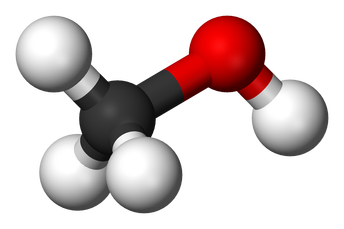
\includegraphics[scale=0.5]{DocumentFigures/Figures/metan.png}
\caption{Ball and stick model of methanol.\cite{CMy}}
\end{figure}


\begin{equation}
\begin{pmatrix}
36.9 & 33.7 & 5.5 & 3.1 & 5.5 & 5.5\\
33.7 & 73.5 & 4.0 & 8.2 & 3.8 & 3.8\\
5.5 & 4.0 & 0.5 & 0.35 & 0.56 & 0.56\\
3.1 & 8.2 & 0.35 & 0.5 & 0.43 & 0.43\\
5.5 & 3.8 & 0.56 & 0.43 & 0.5 & 0.56\\
5.5 & 3.8 & 0.56 & 0.43 & 0.56 & 0.5\\
\end{pmatrix}
\end{equation}

As we know, the building atoms of methanol are four atoms of hydrogen, one carbon atom and one oxygen atom. The Coulomb matrix is invariant with respect to translation, rotation and permutation. In the matrix above, the first row represents carbon that interacts with all the other atoms. The second row corresponds to oxygen and the remaining rows correspond to hydrogen. The matrix is perfectly symmetric, meaning that every corresponding row is equal to every corresponding column.


\subsection{Atomization energy and enthalpy of atomization}

Atomization energy is the quantity that accompanies the total separation of all atoms in a chemical substance (either a chemical compound or a chemical element). It is related to a physico-chemical parameter known as enthalpy of atomization which is the enthalpy change of the total seperation of the atoms. It is often represented by the symbol $\Delta H_{at}$. The associated standard enthalpy is known as standard enthalpy of atomization in units of $\frac{kJ}{mol}$ at 289 K and 1 atmosphere of pressure.

Below is the short description of how one can calculate the atomization energy of a given molecule:

\begin{itemize}
    \item Calculate the total energy for the isolated atoms of the given molecule;
    \item Calculate the total molecule energy;
    \item Subtract the energies of the atoms from the total molecule energy to obtain the atomization energy.
\end{itemize}

\subsection{Spectroscopy}

% https://www.polymersolutions.com/blog/what-is-spectroscopy/

The term spectroscopy is used to describe tools of analytical techniques in which a range of frequencies is applied to matter to obtain spectra of these materials in a form of a graph. The spectra of a matter of interest are gathered by the relationship of frequencies of electromagnetic waves with the matter. Comparing the difference spectra allows the pinpointing of differences between them. Spectroscopy methods allow us to study the structure of a matter in a noninvasive way. We can use machines that grant us precise results e.g IR spectroscopy \cite{maszyny}, but as an alternative let us see what can the topic of artificial intelligence give us in the long term.

\chapter{Machine learning and its principle of working}


\section{Artificial intelligence}

In 1950 Alan Turing started wondering: "Can a machine think like a human?". He laid out the fundamental idea and redefine a question for it to become much easier to precise in a language of machines, namely:"Can a machine imitate and convince other human being that it is also a human?". This question has become a really important idea known as Turing's Test. A human judge asks questions to a person or a machine in the next room. If the machine can convince the judge that it is indeed the human, the machine passes this test. In 1943 Warren McCulloch and Walter Pitts studied how the biological brain works, they proposed the first concept of a simplified brain cell, McCulloch-Pitts (MCP) neuron. Biological neurons create a network of interconnected nerve cells and they use them to send electrical and chemical signals so there is a clear input and a binary output for those signals.\cite{neuron}
The AI research officially started in 1956 at the Dartmouth Conference where a term "artificial intelligence" was created. It was necessary to combine efforts in cybernetics, automata theory, and complex information processing in order to study how can machines think.\cite{histAI}

In 1958, there was some kind of - as was being thought that time -  effort made by Frank Rosenplatt.He published the first concept of the perceptron learning rule based on the MCP neuron model. His proposition of an algorithm was simple, the weight coefficients are multipled by features and the decision is made, the neuron either fires or it doesn't.\cite{raschka}. This gave the birth of certain techniques that are called machine learning.


\begin{figure}[h!]
\centering
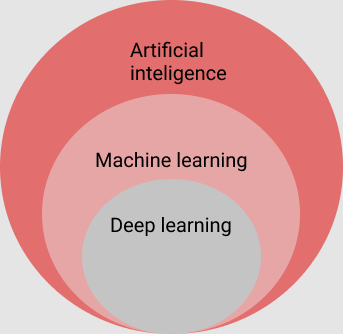
\includegraphics[scale=0.5]{DocumentFigures/MyFigures/zbiorki.png}
\caption{AI, machine learning and deep learning as a set}
\end{figure}



\section{Machine learning}

Algorithms that are trained in machine learning have a major goal: given the massive amounts of data an algorithm has to find patterns and connections in the features in order to make a decision or a prediction. If the choice of an algorithm is suitable enough for a given problem then the algorithm will learn better and will give more accurate predictions. Nowadays, it is hard to not experience machine learning around us every day. Powerful recommendation systems are built using ML models when we search for a song that seems interesting to us. Voice assistants can make a call or schedule a meeting if we tell them to do so. Vacuum cleaners learn all the paths to become optimiezd for cleaning. It is harder and harder for spam to land on our e-mail box. Medicians use image analysis sytems to make a precise diagnosis. Not to mention the rise of self-driving cars which can move us from point A to point B without our interuption. 


\section{Types of machine learning}

\subsection{Supervised machine learning}

Supervised learning requires a labeled dataset. We train our model on the labeled and known. Supervised machine learning requires less training data than other machine learning methods and makes training easier because the results of the model can be compared to actual labeled results.



\subsection{Unsupervised machine learning}

Unsupervised learning is less about automating decisions and predictions, and more about identifying patterns and relationships in data that humans would miss. The unsupervised learning algorithm can analyze huge volumes of emails and uncover the features and patterns that indicate spam 

\subsection{Semi-supervised learning }

Semi-supervised learning offers a happy medium between supervised and unsupervised learning. During training, it uses a smaller labeled data set to guide classification and feature extraction from a larger, unlabeled data set.

\subsection{Reinforcement machine learning}

Reinforcement learning is the training of machine learning models to make a sequence of decisions for a given scenario.
At its core, we have an autonomous agent such as a person, robot, or deep net learning to navigate an uncertain environment. The goal of this agent is to maximize the numerical reward.


\subsection{Deep learning}

Deep learning is a subset of machine learning (all deep learning is machine learning, but not all machine learning is deep learning). Deep learning algorithms define an artificial neural network that is designed to learn the way the human brain learns. Deep learning models use data that pass through multiple neurons, then the weights and biases are applied in each successive layer to continually adjust and improve the outcomes.


\section{Machine learning pipeline}

To be able to build a machine learning model one can summarize the idea in below steps\cite{what_ML_IBM}:

\subsubsection{Selection and preprocessing of a dataset}

Every machine learning model should have a dataset that will be split into two parts: the training set and the testing set. The training set is necessary in order for a model to learn from its mistakes. The test set is used to see how well the model predicts values of interest. Depending on the dataset, it can be labeled, meaning that it has "tags" which combined with certain features can give us solid outputs, other times the data is unlabeled, meaning that the model will have to extract the hidden patterns from the features itself.

\subsubsection{Categorical and numerical data}

When we are dealing with the data, there is a distinction between certain types of the data. The distinction can be summarized as:

\begin{itemize}
    \item Numerical data
    \begin{itemize}
        \item Continuous numerical data
        \item Discrete numerical data
    \end{itemize}
    \item Categorical data
    \begin{itemize}
        \item Ordinal features
        \item Nominal features
    \end{itemize}
\end{itemize}

The numerical data is data points with exact numbers. It can be subdivided into two forms, continuous: such like weight, temperature, salary etc. and discrete: number of students, number of languages spoken. On the other hand, there is a categorical data which represents charateristics such as a hockey player’s position, team, hometown. We can further distinguish the categorical data to ordinal and nominal features: Ordinal features can be sorted or ordered e.g t-shirt sizes, in contrast, nominal features don't imply any order e.g t-shirt color.\cite{raschka}\cite{numericalData}.


\subsubsection{Feature scaling}

Many of the numerical features are unbalanced, for example, there might be times when we will have to process data with different units such as length in kilometers and mass in kilograms. If we put the data as it is we risk the high bias from difference in units. We can use feature scaling methods to give our data the properties of a standard normal distribution that is: mean that is equal to zero and unit variance. Standardization shifts the mean of each feature so that it is centered at zero and each feature has a standard deviation of 1 (unit variance). For instance, to standardize the
$j_{th}$ feature, we can simply subtract the sample mean, $\mu_{j}$ from every training example and then make a division by standard deviation $\sigma_{j}$. Mathematically it presented as follows:

%\begin{equation}
    %\textbf{x'_{j} = \frac{\textbf{x_}_{j} - \mu_{j}}{\sigma_j}}
%\end{equation}

\begin{equation}
    \textbf{x}'_{j} = \frac{\textbf{x}_{j} - \mu_{j}}{\sigma_{j}}.
\end{equation}

In the equation above $\textbf{x}_j$ is a vector with j-th feature values and a standarization is applied to each j-th feature.

\subsubsection{Choosing the right algorithm}

The choice of an algorithm that is going to learn depends on a problem. If we have labeled data then we can proceed to more popular algorithms such as \cite{raschka}:

\begin{itemize}
    \item Regression algorithms: Linear and logistic regression are examples of regression algorithms used to understand relationships in data. Linear regression is used to predict the value of a dependent variable based on the value of an independent variable. Logistic regression can be used when the dependent variable is binary in nature: 1 or 0.
    \item Decision trees: Making a classification based on set of decisions rules. Its advantage comes from a fact that it does not require features to be scaled beforehand.
    \item Instance-based algorithms: Such as k-nearest neighbours, a typical "lazy learner", it doesn't learn a discriminative function from the training data but memorizes the training dataset instead.
\end{itemize}

When we have to deal with unlabeled data we can use for example:

\begin{itemize}
    \item Clustering algorithms:Clustering focuses on identifying groups of similar records and labeling the records according to the group to which they belong. This is done without prior knowledge about the groups and their characteristics using e.g k-means algorithm
    \item Association algorithms:Association algorithms find patterns and relationships in data and identify frequent ‘if-then’ relationships called association rules.
    \item Neural networks:  A deep neural network defines a network with multiple hidden layers, each of which successively refines the results of the previous layer. 
\end{itemize}

\subsubsection{Metric}

We need a tool to compare our results with our expectations from the data. That is why we use different metrics to compare output from different models to be able to find optimized algorithm for given task. Most popular metrics are mean absolute error (MAE)

\begin{equation}
    MAE = \frac{1}{N}\sum_{j=1}^{N}|y_{j} - \hat{y}_{j}|,
\end{equation}

and often mean squared error (MSE):


\begin{equation}
    MSE = \frac{1}{N}\sum_{j=1}^{N}(y_{j} - \hat{y}_{j})^{2},
\end{equation}


where $y_j$ represents the original value and $\hat{y}_j$ represents prediction by a machine learning algorithm.


\subsubsection{Training the algorithms}

Once all the data is prepared and methodology is chosen, we put variables with the data to input. Through the iterations, an algorithm is learning to adjust the weights in order to make the best prediction. Once the algorithm finishes the state of learning, it becomes neccessary to start validation process - using the test set - in order to check how well the model has learnt to predict the data.



\subsection{Model usage and its improvement}

After the training iterations are done, we can test our trained model on a subset of data that we have put to the test set. If we see that our predictions have a large error we have to optimize parameters again and adjust the model again. Sometimes this step means to go back to square one and set new parameters for learning. Below figure can briefly summarise the whole process:

\begin{figure}[h]
\centering

\includegraphics[scale=0.5]{DocumentFigures/MyFigures/strzalkiver.png}
\caption{Example of a machine learning pipeline \cite{MLpipeline} }
\end{figure}




\section{Artificial neural networks}

Artificial neural networks are built on top of artificial neurons. They are inspired by the networksof biological neurons found in our brains. Deep learning is a science that investigates various constructions of
artificial neural networks. They vary from one model to the other, they are efficacious and can be scaled to face hard machine learning problems such as classyfing a large dataset of images (we can think of something like Google Images), controlling speech recognition services (Google Assistant, Apple's Siri, Amazon Alexa), recommending user his favourite movies on Youtube platform or beating an opponent in a chess game.\cite{aurelion}\cite{DeepLearningChess}. It is valuable to stop for a second and to really think why the interest in artificial neural networks will have a huge impact in the nearby future: 
 
\begin{itemize}
    \item We live in times of vast data coming from different sources, it is proven in an AI field that ANNs often outmatch other machine learning techniques when it comes to complex problems.
    \item Thanks to Moore's law ( the number of transistors on an affordable CPU would double every two years \cite{intel}) training of ANN has become achievable due to increased computers' performance. The gaming industry pressurizes the hardware market to be in a state of constant high-end solutions, what is more, cloud computing allowed many users to experiment on ANNs without the worries about their PC components.
    \item The training algorithms have been reinforced. They are similiar to the previous ones from 90s but the reinforcements have made a great impact.
    \item With the increasing knowledge of people about ANNs, there seems to be increase in funding for research, this implies steady progress and thus we shall see new revolutionary products.
\end{itemize}




They can also be called units that are placed in a particular way in a series of layers, each neuron is connected in the network and together they compose a system that we know as Artifical Neural Network. Neural networks are commonly composed with input layer, output layer and some hidden layers. The input layer is responsible for loading the data from a dataset that is of our interest. After the data go through the input, there comes in play hidden layers. It is actually up to a creator of the network to say how many hidden layers will the network have. The hidden layers transform the data for a valuable output for the output layer. Finally, the output layer give us a response signal for the data that has been put in the input. 

\begin{figure}[h]
\centering
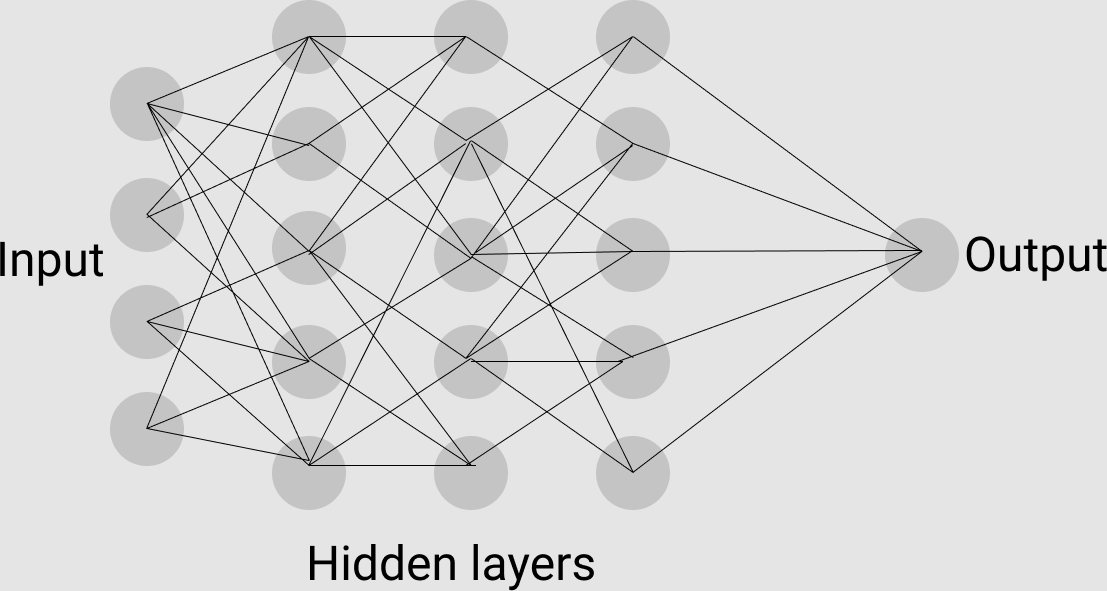
\includegraphics[scale=0.3]{DocumentFigures/MyFigures/sieci2.png}
\caption{Example of a neural network structure \cite{NNSchematic}}
\end{figure}

\section{Single layer neural network}

\subsection{Mathematical principles of Perceptron}

We can put a concept of artificial neuron as a simple binary classification task. The first class is $1$, and the second $-1$.We define a decision function $\phi(z)$ that takes a linear combination of input values $\textbf{x}$ and a weight vector $\textbf{w}$ and it is written as a scalar product of $\textbf{x}$ and $\textbf{w}$, namely:


\begin{equation*}
    z = \textbf{w}^{T}\textbf{x},
\end{equation*}

A decision function makes its prediction using a threshold $\theta$:

\begin{equation}
    \phi(z) = 
\begin{cases}
     1  & \text{if } z \geq \theta, \\
-1  & \text{otherwise.}
\end{cases}
\end{equation}

If we rearange the terms and define a weight-zero as $w_{0} = - \theta$ and $x_{0} = 1$ we can write $z$ as:

\begin{equation*}
    z = w_{0}x_{0} + w_{1}x_{1} + ... + w_{m}x_{m} = \textbf{w}^{T}\textbf{x}.
\end{equation*}

After this operation we write $\phi(z)$ as:

\begin{equation}
    \phi(z) = 
\begin{cases}
     1  & \text{if } z \geq 0, \\
-1  & \text{otherwise.}
\end{cases}
\end{equation}


The negative threshold is often called the bias unit.\cite{raschka}

\subsection{Learning rule of the perceptron}


The whole idea of a learning rule for perceptron can be summarised in a simple manner:

\begin{enumerate}
    \item First, generate random numbers for weights or initialize weights as $0$ from the start
    \item For every training example $\textbf{x}^{(i)}$:
    \begin{itemize}
        \item Compute the output value $\hat{{y}}$ 
        \item Update the weights according to update rule
    \end{itemize}
\end{enumerate}

\subsection{ADAline}

To understand the concept of multilayer neural networks let us begin with simple single layer neural network to show from first principles how a neural network behaves on its fundamental level. One can treat Perceptron as a single layer neural network. In this section we will extend the notion of Perceptron, an improvement called Adaline (ADAptive LInearNEuron) published by Bernard Widrow and his doctoral student Tedd Hoff \cite{adaline}.

The main difference between Rosenblatt's perceptron learning rule and Adaline is the update of weights. The weights are updated using a linear function also called activation function ( crucial concept for deep learning methods) instead of being updated by a unit step function. The activation function in Adaline is written as $\phi(z)$ which is just:


\begin{equation}
    \phi(z) =  \phi(\textbf{w}^{T} \textbf{X}) = \textbf{w}^{T} \textbf{X}.
\end{equation}

However, the algorithm still needs  a threshold function to predict the final output, linear function only learns the weights.

\section{The Multilayer Perceptron and Backpropagation}

A multilayer perceptron is created with one input layer, one or more layers of threshold logic unit (a logic unit that computes a weighted sum of its inputs $z$ and then applies a step function to that sum to make a prediction) called hidden layers, and one end layer called the output layer. If an ANN is built with a deep stack of hidden layers, it is called a deep neural network (DNN). It was a problem for many researchers to find a way to train multilayer perceptron. In 1986, Rumelhart, Hinton and Ronald published their paper \cite{rumelhart1985learning} where they introduced the concept of backpropagation training algorithm which is nowadays used on a regular basis. It is the combination of Gradient Descent and a concept of automatic differentiation - automatical computing of gradients.


\subsection{Gradient Descent}

Main problem for a machine learning algorithm is a defined objective function which we want to optimize while the algorithm is training. This objective function is often a cost function subject to mathematical programming of minimization. Let us define the cost function $J$, to learn the weights as the sum of squared errors (SSE):

\begin{equation}
    J(\textbf{w}) = \frac{1}{2}\sum_{i}^{}(y^{i} - \phi(z^{(i)}))^{2}.
\end{equation}

In comparison to the single layer perceptron, this cost function is differentiable and it is convex. All these implies that we can use a powerful algorithm called gradient descent that we can conceptually visualize in the below picture:

\begin{figure}[h]
\centering
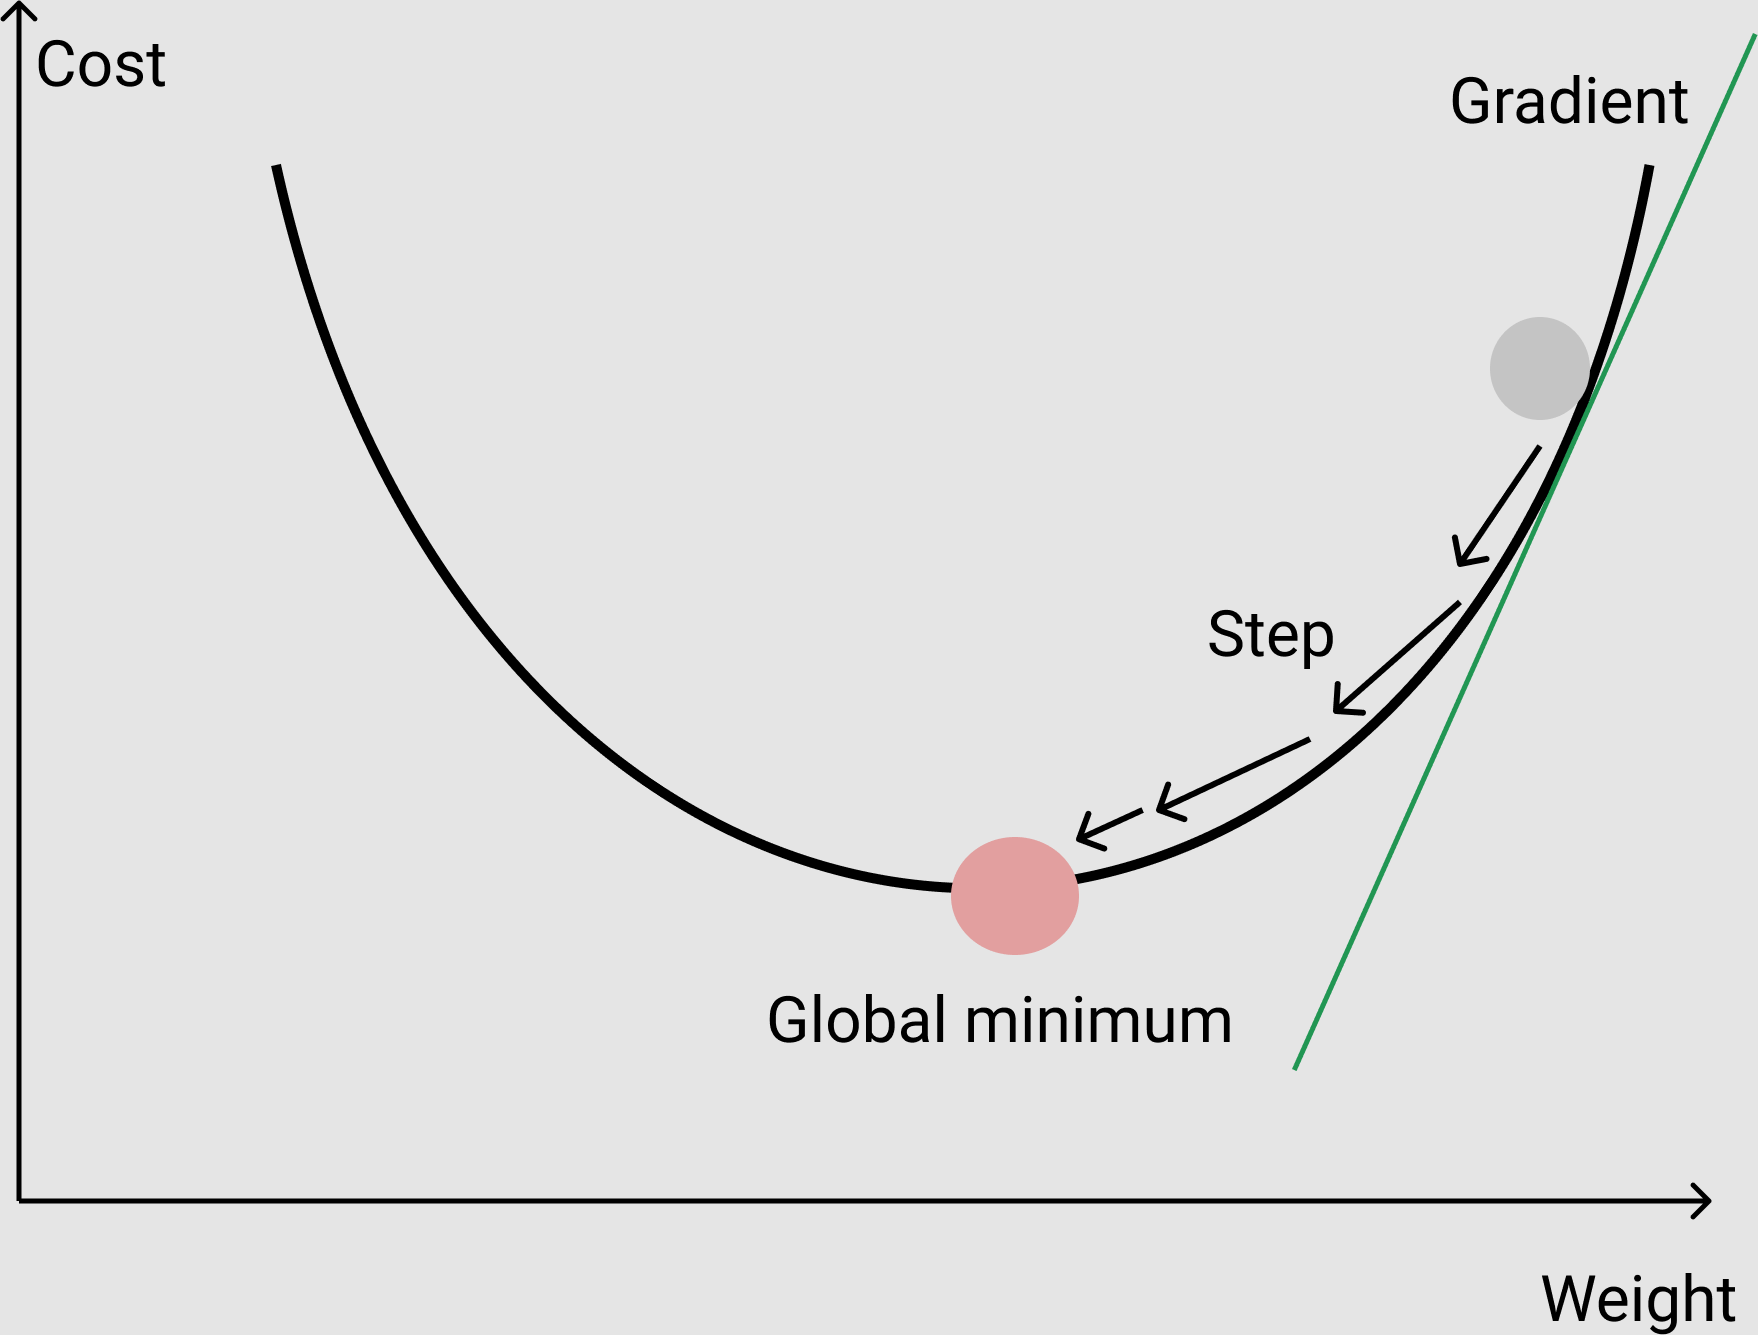
\includegraphics[scale=0.15]{DocumentFigures/MyFigures/MyGradientDescent.png}
\caption{Gradient descent \cite{gradient}}
\end{figure}

After each iteration we want to go in the opposite direction of the gradient, where the step size is coming from the learning rate and the slope of the function. The rule of weight update is:

\begin{equation}
    \textbf{w} := \textbf{w} + \Delta \textbf{w},
\end{equation}

where:

\begin{equation}
    \Delta \textbf{w} = - \eta \nabla J(\textbf{w}).
\end{equation}

Now let us quickly derive the gradient descent for SSE \cite{raschka}:

\begin{equation}
\begin{aligned}
\nabla J(\textbf{w}) = \frac{\partial J}{\partial w_j} = \frac{\partial }{\partial w_j} \frac{1}{2} \sum_{i}^{}(y^{(i)} - \phi(z^{(i)}))^{2}  \\
       = \frac{1}{2} \frac{\partial }{\partial w_j} \sum_{i}^{}(y^{(i)} - \phi(z^{(i)}))^{2}  \\
      = \frac{1}{2}  \sum_{i}^{}2(y^{(i)} - \phi(z^{(i)}))\frac{\partial }{\partial w_j}(y^{(i)} - \phi(z^{(i)}))  \\
      = \sum_{i}^{}\big(y^{(i)} - \phi(z^{(i)})\big)\frac{\partial}{\partial w_{j}}\Big(y^{(i)} - \sum_{i}^{}(w_{j}^{(i)}x_{j}^{(i)}) \Big)\\
      = - \sum_{i}^{}(y^{(i)} - \phi(z^{(i)}) \cdot x_{j}^{(i)}.  
\end{aligned}
\end{equation}

\subsection{Stochastic Gradient Descent}

If we have a large piles of data it is hard to use Gradient Descent especially because it can be computationally heavy to reevaluate the whole training dataset each time we take a step toward the global minimum.

There is a popular alternative for GD, Stochastic Gradient Descent, sometimes also called iterative or online gradient descent. The difference is this: Instead of updating the weights based on the sum of the accumulated errors over all training examples , $\textbf{x}^{(i)}$:

\begin{equation}
    \Delta \textbf{w} = \eta \sum_{i}^{}(y^{(i)} - \phi(z^{(i)}) \cdot \textbf{x}^{(i)},
\end{equation}


we just update the weights for each example:

\begin{equation}
    \eta (y^{(i)} - \phi(z^{(i)}) \cdot \textbf{x}^{(i)}.
\end{equation}

The strength of stochastic gradient descent is reaching convergence much faster than the "regular" gradient descent, after all, we update the weights more frequently. Each gradient is evaluated on a single example therefore there is the error surface is noiser than in GD which has its advantage when it comes to escaping local minima. It is worth to mention that to get accurate results one must shuffle the dataset for every iteration to prevent cycles and one must present the data in a random order. \cite{raschka}


\subsection{Automatic differentiation}


Calculating the derivatives by hand in gradient descent algorithm would be quite tedious especially when we have many iterations of our model. Derivatives in computing can can be calculated by four main methods:

\begin{itemize}
    \item working out derivatives manually and coding results into computer;
    \item  numerical differentiation;
    \item symbolic differentiation using computer algebra;
    \item automatic differentiation;
\end{itemize}


While we could figure out derivatives manually and then put them into a computer and this would get rid of problems with approximation errors and make the derivatives stable in comparison with numerical differentiation, this method has an unavoidable weakness, it is prone to human error and as was said before can become tiresome after a while. Symbolic differentiation could have been a sweet spot between both previous methods but can result with the problem of "expression swell".

The automatic differentiation (AD) gives another look at the problem. It consistently applies the chain rule of calculus to calculate a "flow" of derivatives. Given a series of computations $y = f(g(h(x)))$ with input $x$ and output $y$ we broke this into a series of steps: \cite{raschka}

\begin{itemize}
    \item $u_{0} = x$;
    \item $u_{1} = h(x)$;
    \item $u_{2} = g(u_{1})$;
    \item $u_{3} = f(u_{2}) = y$;
\end{itemize}

Then the derivative $\frac{dy}{dx}$ can be computed in two different ways:

\begin{itemize}
    \item forward accumulation: $\frac{du_{3}}{dx} = \frac{du_{3}}{du_{2}}\frac{du_{2}}{du_{0}}$
    \item backward accumulation: $\frac{dy}{du_{0}} = \frac{dy}{du_{1}}\frac{du_{1}}{du_{0}}$
\end{itemize}






It is important to remember that automatic differentiation is not numerical differentiation. The standard finite difference formula uses a definition:

\begin{equation}
    \frac{d f(x)}{dx} = \lim_{h \to 0} \frac{f(x + h) - f(x)}{h}.
\end{equation}

While it is easy to implement it is prone to truncation and round-off errors. AD is also not symbolic differentiation such as we see in CAS programs (computer algebra system) like Mathematica, Maple, Maxima, Sage, Matlab. Symbolic results allow for analytical methods to solve a problem but one must take into account that expressions can get exponentially larger through differentiation. \cite{baydin2014automatic}


\subsection{Backpropagation}

Now we can proceed to the heart of the ANNs - backpropagation algorithm. To sum it up - it uses Gradient Descent with automatic differentiation, meaning that: there are two phases of data flow (two passes through the network one forward and one backward). The backpropagation computes the gradient of an error with regard to every single model parameter. Then it performs a Gradient Descent and the whole process is continued until the network converges. Below we list the process of backpropagation:


\begin{itemize}
    \item The gradient descent goes over all the training set multiple times. Each pass is called an epoch;
    \item Each mini-batch is sent to the input layer and then to the first hidden layer. Then there is a computation of neurons in this layer, the result is transported to another layer, the output is computed and then it is sent to another layer and so on untill the output layer is finally reached. This is actually a process of making predictions, but intermediate results are upholded beacuse they will be needed for the backward pass;
    \item After forward pass, the algorithm measures how far from prediciton it was, the loss function compares predicted values from the network with actual values and then it returns some measure of the error;
    \item Then the chain rule is used to estimate how much each output connection contributed to the error;
    \item The algorithm works backward using chain rule again to estimate how much of error contributions came from connection in the layer below (backpropagation);
    \item On the last step, the algorithm uses Gradient Descent to make corrections to weights, using the gradient that it has calculated previously \cite{aurelion};
\end{itemize}


\section{Activation function}

Activation functions are used to decide if a neuron should be activated or not. Essentialy, they transform input signals to output signals. Below, are presented common activation functions used heavily in the industry as well as in research:


\begin{itemize}
    \item One of the more popular activation function is ReLU (rectified linear unit). Given an element $x$, the function is defined as the maximum of that element and $0$, $ReLU(x) = \max(x, 0)$;
    \item The sigmoid function $f(x) = \frac{1}{1 + \exp(-x)}$ is defined as $f: \mathbb{R} \rightarrow (0, 1)$. It is commonly used in a more classic machine learning algorithms such as logistic regression;
    \item Similiar to sigmoid activation function, the $\tanh(x)$ function exhibits point symmetry about the origin of the coordinate system;
\end{itemize}



\chapter{Software}

\section{Software tools}

This section's purpose is solely to show what types of tools where used when writing the implementation of a theory. First we will describe Python programming language and its momentum in the world of science and then we will give some details about libraries that were used in a code.

\subsection{Python }

Python \cite{Python} is a programming language created in 1991 by Guido van Rossum. It is not a compiled language, rather it has an interpreter that helps it execute instructions without a need for previous compiling into a machine-language instructions. It is a multi-paradigm languauge, meaning that it doesn't make a programmer use a specified programming paradigm, one can actually focus on solving a given problem instead of worrying about certain paradigm's rules. Since Python is object-oriented, it organizes its structure not by using logic and functions but it treats everything as an object. An object can be defined as a data field that has unique attributes and behavior. The strength of a Python language comes from a fact that it has a really easy syntax making a point of readability and a large number of general and highly specialized libraries. A natural implication from this fact stems that one can focus on writing code efficiently and quickly in comparison to other programming languages. It is not surprising then that Python gained a lot of popularity in the scientific world. A scientist doesn't have to worry about some unpleaseant things when creating his/her software e.g manual memory management, he/she just strictly starts to implement a given problem. The community of Python constantly tries to improve the language and serves its support for new users.

\subsection{NumPy}


NumPy \cite{numpy} is a library made for scientific computing in Python. It provides a multidimensional array object, a special type of matrix objects and variety of different implementations of fast operations on arrays like linear algebra methods, discrete Fourier Transforms, statistical operations, random simulations and more. At the top of hierarchy in NumPy library is object called \emph{ndarray}. This encapsulates n-dimensional arrays of homogeneous data types, with many operations being performed in compiled code for performance. The strenght of NumPy comes from a fact that it does all of its operations on vectors "behind the scenes" using C programming language. A vectorized code has its advantages such that:

\begin{itemize}
    \item It is easier to read;
    \item It is
    possible to achieve same outcomes with fewer lines of code so there is less probability for a mistake;
    \item It maintains reasonable computational complexity by not using loops;
\end{itemize}


\subsection{Keras}

Keras \cite{Keras} is an API (Application Programming Interface) written in Python for a much popular machine learning platform - TensorFlow. It gives a kind of interface for TensorFlow to quickly and accurately implement ideas and machine learning solutions. It was created with a concept of fast experimentations on data in opposite to TensorFlow which gives much more power to a user in developing highly efficent algorithms. We can think of Keras as a higher layer of TensorFlow: It gives us specific tools and options to quickly create and develop a model using exceptionally fast and powerful iterations of automatic differentiation. Keras can be run on TPU (Tensor Processing Unit) or on large clusters of GPUs (Graphics Processing Unit) and it supports exports to run models in a browser or on a mobile device. The structure of Keras is divided between layers and models. The simplest type of model is the Sequential model, a linear stack of layers. 

\subsection{TensorFlow}

TensorFlow \cite{tf} is an open source library for developing and training machine learning models. It was created by Google company using Python as an API for execution code written in C++ for maximum performance. It allows developers to create graph structure, where data flow through graphs and each graph represents a mathematical operation. The graphs are connected by a multidimensional arrays which is treated as a tensor. All the values in this tensor hold indentical data type with a known shape ( dimensions ). The power of Tensorflow comes from its pipeline when solving a given problem using machine learning, meaning:

\begin{itemize}
    \item Preprocessing of the data;
    \item Building the model;
    \item Training and estimating the model;
\end{itemize}

Finally, a significant feature of TensorFlow is the TensorBoard. The TensorBoard enables to monitor graphically and visually what TensorFlow is doing.

\subsection{Scikit-learn}

Scikit-learn \cite{sklearn} is an open source machine learning library for Python programming language as well as a simple yet powerful data analysis tool. It was created as a layer between NumPy, Matplotlib and SciPy focusing on classical ML methods rather than reinforcement learning. It contains many tools helpful in solving regression, classification, clustering and dimensionality reduction problems. The project was started in 2007 as a Google Summer of Code project by David Cournapeau. Later that year, Matthieu Brucher started work on this project as part of his thesis. Scikit-learn has a nice infrastructure in composing the pipeline of project, it has many built-in machine learning algorithms and models called estimators, each estimator can be fitted to some data using its fit method. There is also a place for transformers, objects used for pre-processing the data before they go to a predictor. Together, transformers and estimators give nicely shaped structure for producting a fully developed model in just a few lines of code. 


\subsection{SciPy}

The SciPy \cite{scp} library is one of the core packages that make up the SciPy stack. It provides many user-friendly and efficient numerical routines, such as routines for numerical integration, interpolation, optimization, linear algebra, and statistics. It creates an eco-system for making scientific calculations easier and it splits between four different packages:

\begin{itemize}
    \item Python;
    \item NumPy;
    \item SciPy library;
    \item Matplotlib;
\end{itemize}


\subsection{Matplotlib}

Matplotlib \cite{mpl} \cite{Hunter:2007} is a library for making fully customized plots in Python either 2D or 3D. Although historically the library was written purely in Python, nowadays it is fully equiped with NumPy vectorized arrays. This combination assures that bars, plots, charts, animations, etc. can always be handled despite of relatively large data chunks. In just a few lines of code one can simply code a clear and concise plots or he/she can experiment with richness of modules, functions and classes to present fancy architectures. The architecure of Matplotlib is roughly divided in three parts:

\begin{itemize}
    \item he pylab interface is the set of functions provided by matplotlib.pylab which allow the user to create plots;
    \item he set of classes that do the heavy lifting, creating and managing figures, text, lines, plots and so on;
    \item he backends are device-dependent drawing devices, aka renderers, that transform the frontend representation to hardcopy or a display device;
\end{itemize}



\subsection{Pandas}

Pandas \cite{pandas} is an open source data analysis and manipulation tool, built on top of the Python programming language. It has been in development since 2008 and is \emph{de facto} standard in industry with a strong position to be one of the best managed open source project. Pandas has everything a data scientist needs in his/her job. Pandas comes with a DataFrame object that allows a user to manipulate data with integrated indexing. It has an in-built data structures like CSV and text files, Microsoft Excel, SQL databases, and the fast HDF5 format for saving or reading data. If there is a necessity for an optimized, fast and efficient code, Pandas uses critical code paths written in Cython or C. Python with pandas is in use in a wide variety of academic and commercial domains, including Finance, Neuroscience, Economics, Statistics, Advertising, Web Analytics, and more. Pandas aims to be the fundamental high-level building block for doing practical, real world data analysis in Python.




\part{Applications}

\chapter{Implementation of the ML algorithm}

\section{Dataset}

The dataset that has been used in implementation of a network was taken from \cite{dataset}.The whole credit of using this data goes to \cite{blum} \cite{rupp}. It is a subset of a much broader data set, namely GDB-13 which contains close to one billion stable and synthetically accessible organic molecules. It is important to note that QM7 dataset has molecules that do not exceed 23 atoms in accordance to their structure. The whole dataset has 7165 molecules with their Coulomb's matrices calculated beforehand. The atomization energies are in SI units of kcal/mole in the range between $-800$ to $-2000$ kcal/mole.The structure of QM7 is as follows:

\begin{itemize}
    \item Array X: It represents the molecules and their respective Coulomb's matrices having the shape (7165 x 23 x 23), this array is treated as an iput for neural network.
    \item Array T: It represents the atomization energies of the molecules having the shape (7165).
    \item Array P: It represents a set of data used for cross validation.
    \item Array Z: It represents the value of atomic charge used for calculating Coulomb's matrix.
    \item Array R: It represents the cartesian coordinate of each atom in the molecules.
\end{itemize}

\section{Data preprocessing}

By using the below code we can preview first records of the data that will be put into the MLP algorithm:

\begin{verbatim}
    X = dataset["X"]
    y = dataset["T"].T

    X[:3]
    y[:3]
\end{verbatim}

And see how the data look like in the array for y - dependent variable:

\begin{verbatim}
    array([[-417.96],
       [-712.42],
       [-564.21]], dtype=float32)
\end{verbatim}

And independent variable X:

\begin{verbatim}
    array([[[36.858105 ,  2.9076326,  2.907612 , ...,  0.       ,
          0.       ,  0.       ],
        [ 2.9076326,  0.5      ,  0.29672  , ...,  0.       ,
          0.       ,  0.       ],
        [ 2.907612 ,  0.29672  ,  0.5      , ...,  0.       ,
          0.       ,  0.       ],
        ...,
        [ 0.       ,  0.       ,  0.       , ...,  0.       ,
          0.       ,  0.       ],
        [ 0.       ,  0.       ,  0.       , ...,  0.       ,
          0.       ,  0.       ],
        [ 0.       ,  0.       ,  0.       , ...,  0.       ,
          0.       ,  0.       ]],

       [[36.858105 , 12.599944 ,  2.9019997, ...,  0.       ,
          0.       ,  0.       ],
        [12.599944 , 36.858105 ,  1.4731166, ...,  0.       ,
          0.       ,  0.       ],
        [ 2.9019997,  1.4731166,  0.5      , ...,  0.       ,
          0.       ,  0.       ],
        ...,
        [ 0.       ,  0.       ,  0.       , ...,  0.       ,
          0.       ,  0.       ],
        [ 0.       ,  0.       ,  0.       , ...,  0.       ,
          0.       ,  0.       ],
        [ 0.       ,  0.       ,  0.       , ...,  0.       ,
          0.       ,  0.       ]],

       [[36.858105 , 14.261827 ,  1.503703 , ...,  0.       ,
          0.       ,  0.       ],
        [14.261827 , 36.858105 ,  2.9250205, ...,  0.       ,
          0.       ,  0.       ],
        [ 1.503703 ,  2.9250205,  0.5      , ...,  0.       ,
          0.       ,  0.       ],
        ...,
        [ 0.       ,  0.       ,  0.       , ...,  0.       ,
          0.       ,  0.       ],
        [ 0.       ,  0.       ,  0.       , ...,  0.       ,
          0.       ,  0.       ],
        [ 0.       ,  0.       ,  0.       , ...,  0.       ,
          0.       ,  0.       ]]], dtype=float32)
\end{verbatim}


This is how the data with coulomb matrix looks like (first entry of the data, 23 x 23 coulomb matrix) as well as the target variable that we want to predict:

\begin{figure}[h!]
\centering
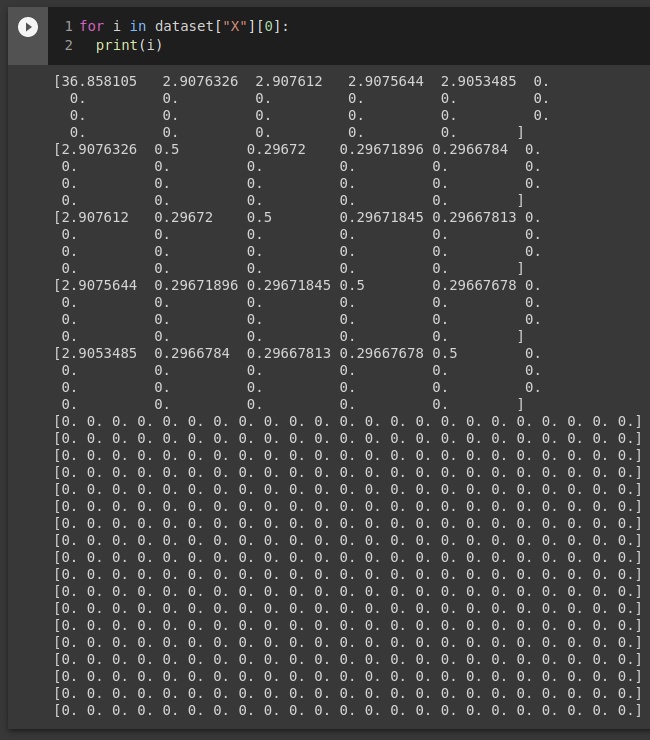
\includegraphics[scale=0.5]{DocumentFigures/MyFigures/input_data_CM.png}
\caption{Screenshot of data - the input variable}
\centering
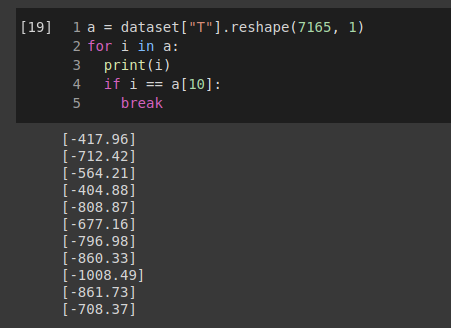
\includegraphics[scale=0.8]{DocumentFigures/MyFigures/target_variable.png}
\caption{Screenshot of data - the target variable}
\end{figure}

\section{Google colaboratory platform}

Since deep learning methods can be highly sensitive to hardware of a computational unit, we will use Google Colaboratory (Colab), the free platform for typing and executing Python code along with neccessary libraries. Using Colab will have an advantage of being portable, one can open a web browser and does not have to worry about performance speed and computing resources. Strengths of Colab come from those facts:

\begin{itemize}
    \item It has pre-configured environment so a user does not have to manually pre-set every setting connected to Python ecosystem.
    \item It gives free (up to 12 hours) access to using GPU (Graphical Processing Unit) so a user does not have to have a PC that comes from high-end technology.
    \item It is portable, the wholde code can be saved and download as a .ipynb file so it can be run later on any device with Python on the board.
\end{itemize}


Below we can see how the code can be compiled using Google environment:

\begin{figure}[h!]
\centering
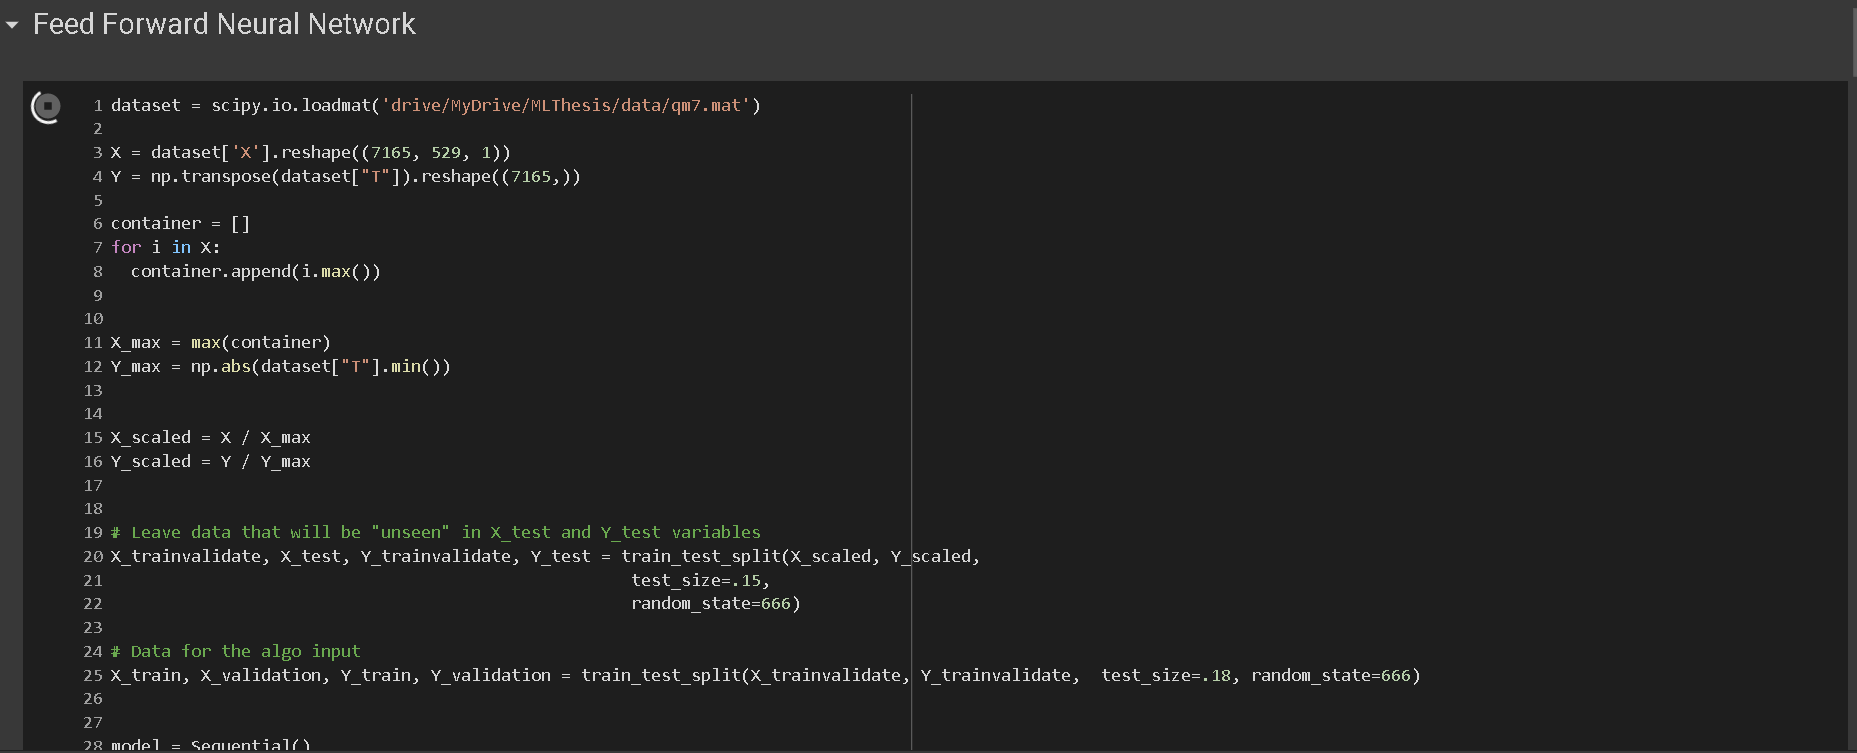
\includegraphics[scale=0.4]{DocumentFigures/MyFigures/feedforwardenvir.png}
\caption{Google Colaboratory Platform - screenshot I}
\end{figure}

\begin{figure}[h!]
\centering
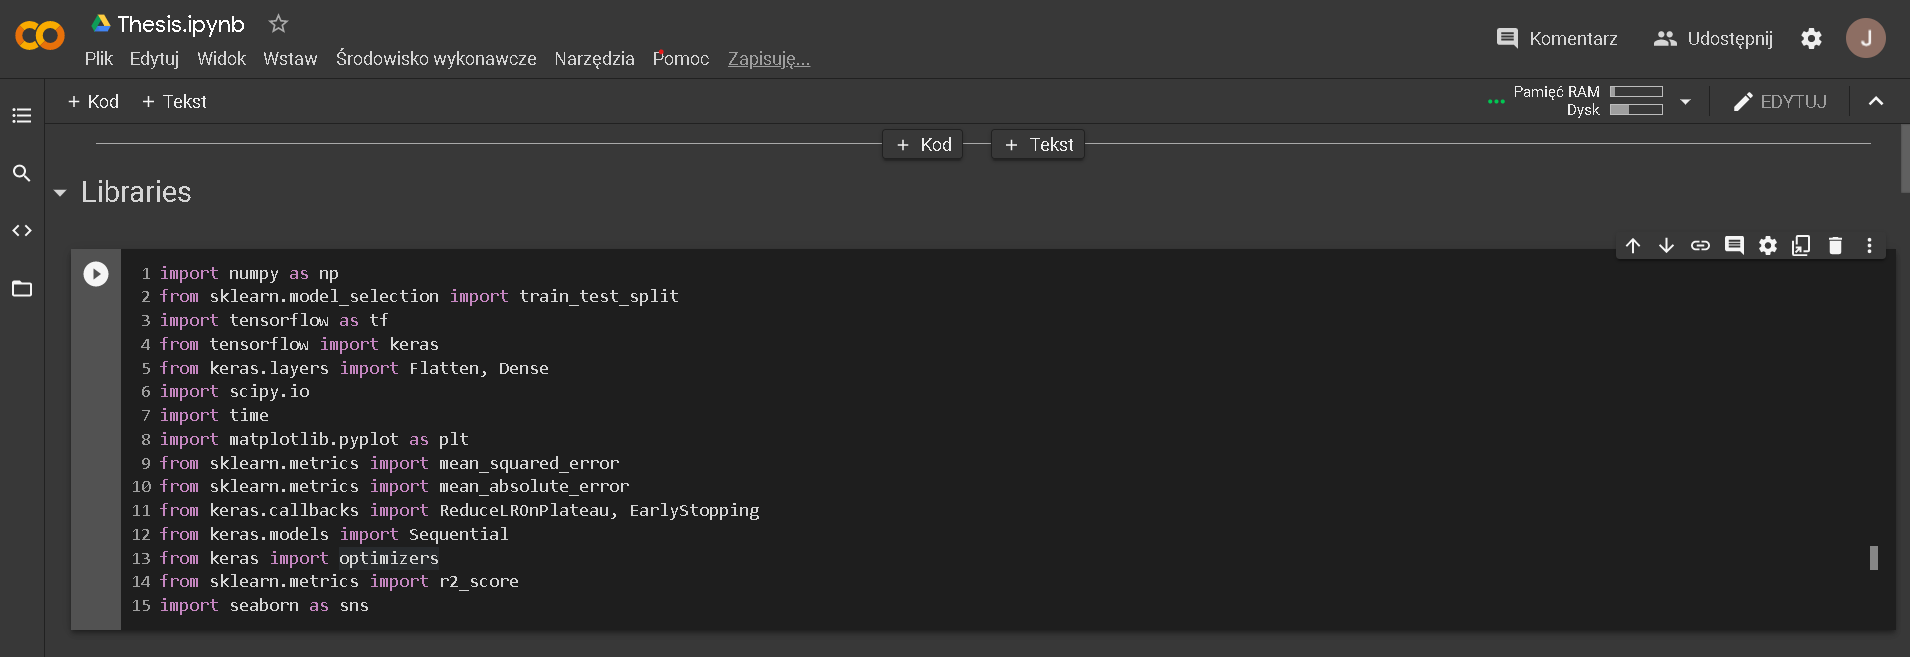
\includegraphics[scale=0.4]{DocumentFigures/MyFigures/ImpotLibrariesEnvir.png}
\caption{Google Colaboratory Platform - screenshot II}
\end{figure}



\section{Pipeline}

\subsection{Importing libraries}

This step is self explanatory. The imports of libraries are neccessary to run the program:

\begin{verbatim}[language=Python]

import numpy as np
from sklearn.model_selection import train_test_split
import tensorflow as tf
from tensorflow import keras
from keras.layers import Flatten, Dense
import scipy.io
import time
import matplotlib.pyplot as plt
from sklearn.metrics import mean_squared_error
from sklearn.metrics import mean_absolute_error
from keras.callbacks import ReduceLROnPlateau, EarlyStopping
from keras.models import Sequential
from keras import optimizers
from sklearn.metrics import r2_score
import seaborn as sns


\end{verbatim}


\subsection{Dataset loading}

We use sci-kit learn library to load our dataset. It is written as .mat file ( meaning that it was generated in MATLAB environment). By using loadmat() method we convert the data to numpy array:

\begin{verbatim}[language=Python]


dataset = scipy.io.loadmat('drive/MyDrive/MLThesis/data/qm7.mat')


\end{verbatim}

\subsection{Scaling and reshaping}

After we have loaded the dataset. We first begin by reshaping the input variable $X$ and target variable $Y$ to dimensions acceptable by ANN. Since $X$ is composed of  $23 \times 23$ matrices we "flatten" every matrix from $X$ to $529 \times 1$. We are also reshaping $Y$ so we can represent it as a row vector.

We use one of the simplest methods of data scaling, taking maximum value of both sets and dividing each entry by this maximum value.

\begin{verbatim}[language=Python]


X = dataset['X'].reshape((7165, 529, 1)) 
Y = np.transpose(dataset["T"]).reshape((7165,))

container = []
for i in X:
  container.append(i.max())
  

X_max = max(container)
Y_max = np.abs(dataset["T"].min())


X_scaled = X / X_max
Y_scaled = Y / Y_max


\end{verbatim}

\subsection{Splitting data to training, validation and test sets}

We begin by using the holdout method and we are splitting the data into three parts: a training dataset, a validation dataset, and a test dataset. Test data set vs validation and training data set is split in 80:20 ratio. Same is the split for training and validation.


\begin{verbatim}
# Leave data that will be "unseen" in X_test and Y_test variables
X_trainvalidate, X_test, Y_trainvalidate, Y_test = train_test_split(X_scaled, 
                                                                    Y_scaled,  
                                                    test_size=.20, 
                                                    random_state=666)

# Data for the algo input
X_train, X_validation, Y_train, Y_validation = train_test_split(X_trainvalidate, 
                                                                Y_trainvalidate,  
                                                                test_size=.20, 
                                                                random_state=666)
\end{verbatim}


\subsection{Sequential model}

After the data pre-processing we can go into the structure of a model using Keras sequential model. It is a perfect fit for a situation where each layer has exactly one input tensor and one output tensor where overall, we have a stack of layers. We could not use the sequential model in a following scenario:

\begin{itemize}
    \item There would have been multiple inputs or outputs in the model
    \item Any layer has multiple inputs or outpus
    \item A layer sharing is required for a model to perfom well
    \item There would be a need for non-linear topology
\end{itemize}

We will pass a list of layers to the Sequential constructor contained in variable "model". We will also specify a normal distribution for weights generation. :

\begin{verbatim}

model = Sequential()
kernel_initializer='he_normal'

# 64 -> 128 -> 529 -> Flatten -> 1
model.add(Dense(64, activation='relu', kernel_initializer=kernel_initializer))
model.add(Dense(128, activation='relu', kernel_initializer=kernel_initializer))
model.add(Dense(529, activation='relu', kernel_initializer=kernel_initializer))
model.add(Flatten())
model.add(Dense(1, activation='linear'))
\end{verbatim}


After the above is met, we use compile method to configurate the model for training. Our loss will be measured using Mean Absolute Error (and additional Root Mean Square Error set in metrics variable) and we choose Adam for our gradient descent optimization algorithm with learning rate set to 0.001.

\begin{verbatim}
    
    model.compile(loss='mae',
              optimizer=optimizers.Adam(.001),
              metrics=['mae', tf.keras.metrics.RootMeanSquaredError()])
    
\end{verbatim}




Through the usage of "add" method, we create overall 6 layers with different shapes, we use reLU activation function for the first four layers, then we use "Flatten" function (the whole operation is sketched below) to get our output as a 1-D vector using linear activation function on the output. 


\subsection{Sketch of the model ( layers and flattening)}

\begin{figure}[h!]
\centering
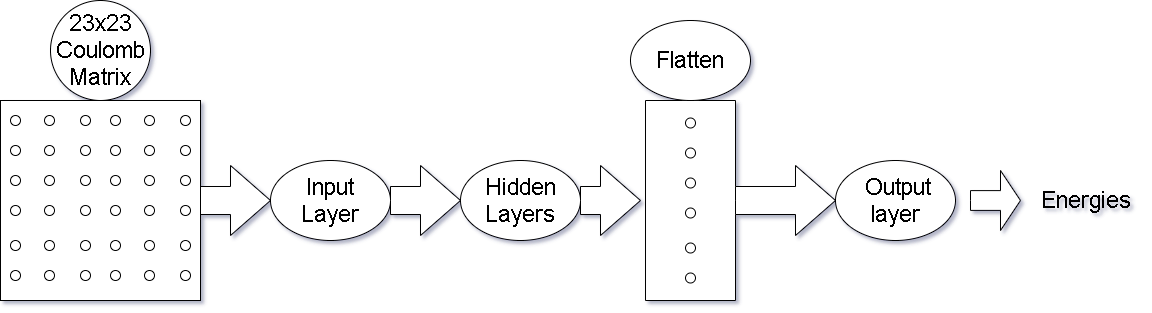
\includegraphics[scale=0.4]{DocumentFigures/MyFigures/FlattenOperatioNNscheme.png}
\caption{Simplified sketch of architecture}
\end{figure}


\section{Training the model}


We begin by using time module to calculate how long will it take for the model to finish training. We use a callback API to make our model more efficient using ReduceLROnPlateau. If the metric stops improving after some specified ("patience" parameter) period of time (epochs) this method will accelerate the convergence of the algorithm by reducing eta parameter by the factor of 0.1.

We set number of epochs to 15 and we initialize training of the model by providing 7 arguments: coulomb matrix train dataset, energies from the train set, batch size of our model, previously specified number of epochs, callback parameter for reducing eta, and validation data. Finally, we print the network summary via summary() method.

\begin{verbatim}[language=Python]

start = time.time()


reduce_eta = ReduceLROnPlateau(monitor='val_loss', factor=0.1, patience=1, verbose=1)

n_epochs = 15

history = model.fit(X_train, Y_train,
                      batch_size=4,
                      epochs=n_epochs, 
                      callbacks=[reduce_eta],
                      verbose=1,
                      validation_data=(X_validation, Y_validation))

model.summary()

end = time.time()

print(f"Training time: {end-start}")
print(f"Number of epochs: {n_epochs}")

\end{verbatim}

\section{Results}


The algorithm was given 15 epochs until it finished training itself and Mean Absolute Error on test dataset yields 23.040 MAE and reaching the last epoch was obtained after 582.57 seconds.

\begin{figure}[h!]
\centering
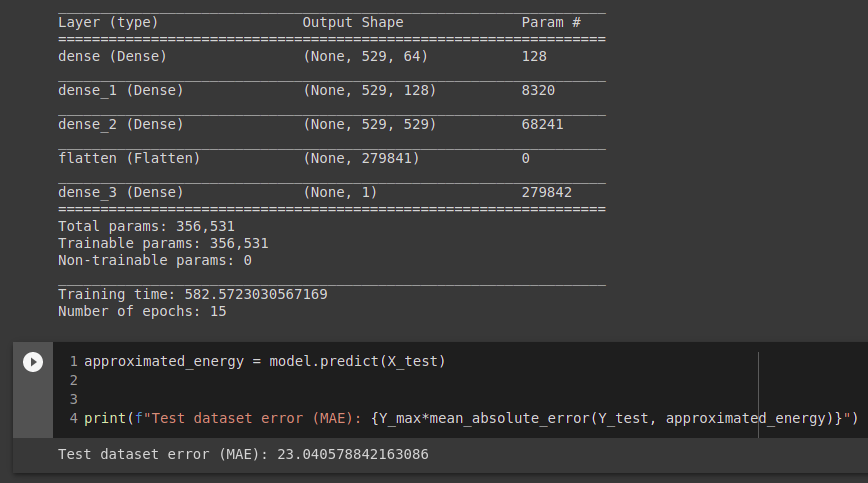
\includegraphics[scale=0.5]{DocumentFigures/ZdjeciaWalidacja/MAEtest.png}
\caption{Summary of the model after all iterations have passed}
\end{figure}




\begin{figure}[h!]
\centering
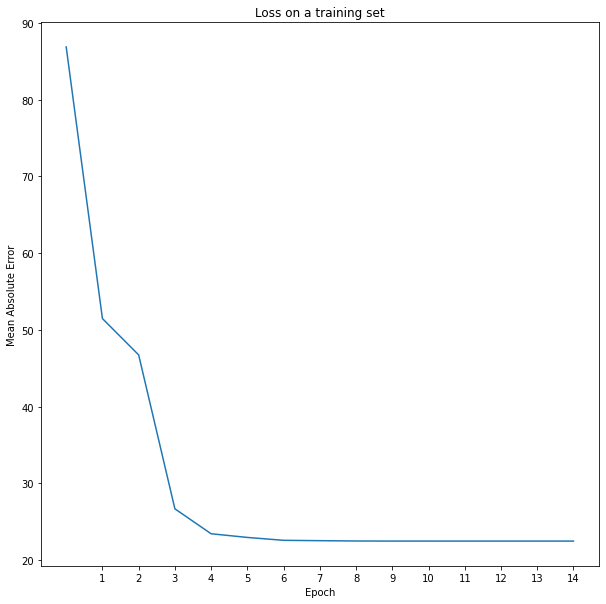
\includegraphics[scale=0.8]{DocumentFigures/ZdjeciaWalidacja/Losstraining.png}
\caption{Plot of loss using Mean Absolute Error on a training dataset}
\end{figure}


\begin{figure}[h!]
\centering
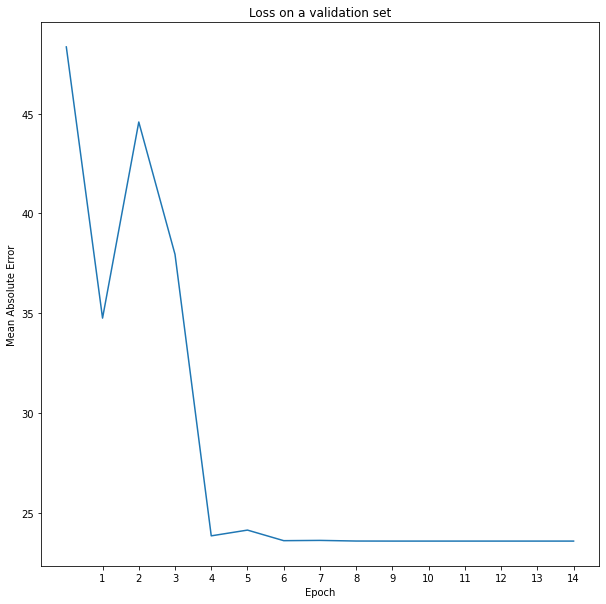
\includegraphics[scale=0.8]{DocumentFigures/ZdjeciaWalidacja/Lossvalidation.png}
\caption{Plot of loss using Mean Absolute Error on a validation dataset}
\end{figure}



\begin{figure}[h!]
\centering
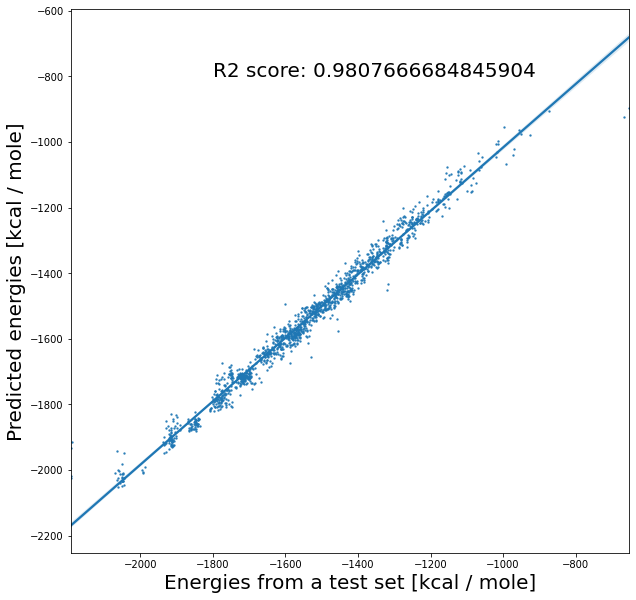
\includegraphics[scale=0.7]{DocumentFigures/ZdjeciaWalidacja/R2test.png}
\caption{R2 score for test dataset}
\end{figure}



\begin{figure}[h!]
\centering
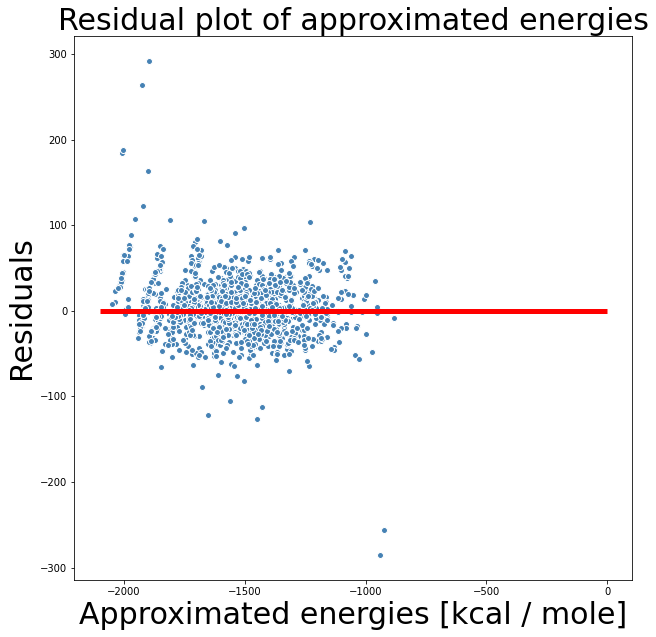
\includegraphics[scale=0.7]{DocumentFigures/ZdjeciaWalidacja/ResidualsTest.png}
\caption{Residual plot for predicted energies}
\end{figure}




\section{Conclusions}

The author of this thesis has described the quantum principles that have been used to calculate chemical quantum parameters such as atomization energy. We can see that algorithm has reached convergence both on training set and validation set implying that it has found the approximated solution (approximated energies) with $23.04$ MAE. The $R^2$ coefficient of determination of the regression analysis gives $0.9769$ which implies that the approximated energies were predicted in a way that they closely resemble the real ones. Residual analysis shows that there are only few outliers and there is not a clear visible pattern constructed from points therefore we can say that the model is able to capture some explanatory information.

It has been shown that Deep Learning methods can be used to solve interesting Physics phenomena in quantum oriented field. What remains is the need to improve the validity of the models and closely approach the chemical and physical accuracy that one can achieve by the experiment.



\appendix
\appendixpage
\addappheadtotoc
\chapter{Implementation of ANN in Python}



\begin{verbatim}

Automatically generated by Colaboratory.

Original file is located at
    https://colab.research.google.com/drive/10gPxt_Np-Q7P-HBprNad8SVtuS9nQyZ0

##Libraries
"""

import numpy as np
from sklearn.model_selection import train_test_split
import tensorflow as tf
from tensorflow import keras
from keras.layers import Flatten, Dense
import scipy.io
import time
import matplotlib.pyplot as plt
from sklearn.metrics import mean_squared_error
from sklearn.metrics import mean_absolute_error
from keras.callbacks import ReduceLROnPlateau, EarlyStopping
from keras.models import Sequential
from keras import optimizers
from sklearn.metrics import r2_score
import seaborn as sns

"""##Feed Forward Neural Network"""

dataset = scipy.io.loadmat('drive/MyDrive/MLThesis/data/qm7.mat')

X = dataset['X'].reshape((7165, 529, 1)) 
Y = np.transpose(dataset["T"]).reshape((7165,))

container = []
for i in X:
  container.append(i.max())
  

X_max = max(container)
Y_max = np.abs(dataset["T"].min())


X_scaled = X / X_max
Y_scaled = Y / Y_max


# Leave data that will be "unseen" in X_test and Y_test variables
X_trainvalidate, X_test, Y_trainvalidate, Y_test = train_test_split(X_scaled, Y_scaled,  
                                                    test_size=.15, 
                                                    random_state=666)

# Data for the algo input
X_train, X_validation, Y_train, Y_validation = train_test_split(X_trainvalidate, Y_trainvalidate,  test_size=.18, random_state=666)


model = Sequential()
kernel_initializer='he_normal'

# 64 -> 128 -> 529 -> Flatten -> 1
model.add(Dense(64, activation='relu', kernel_initializer=kernel_initializer))
model.add(Dense(128, activation='relu', kernel_initializer=kernel_initializer))
model.add(Dense(529, activation='relu', kernel_initializer=kernel_initializer))
model.add(Flatten())
model.add(Dense(1, activation='linear'))


model.compile(loss='mae',
              optimizer=optimizers.Adam(.001),
              metrics=['mae', tf.keras.metrics.RootMeanSquaredError()])



start = time.time()


reduce_eta = ReduceLROnPlateau(monitor='val_loss', factor=0.1, patience=1, verbose=1)

n_epochs = 15

history = model.fit(X_train, Y_train,
                      batch_size=4,
                      epochs=n_epochs, 
                      callbacks=[reduce_eta],
                      verbose=1,
                      validation_data=(X_validation, Y_validation))

model.summary()

end = time.time()

print(f"Training time: {end-start}")
print(f"Number of epochs: {n_epochs}")

"""## Validation"""

approximated_energy = model.predict(X_test)


print(f"Test dataset error (MAE): {Y_max*mean_absolute_error(Y_test, approximated_energy)}")
print(f"Test dataset error (RMSE): {Y_max*mean_squared_error(Y_test, approximated_energy, squared=False)}")

#plt.figure(figsize=(8,8))

loss = np.array(history.history["loss"]) * Y_max
mae = np.array(history.history["mae"]) * Y_max
rmse = np.array(history.history['root_mean_squared_error']) * Y_max
val_loss = np.array(history.history["val_loss"]) * Y_max
val_mae = np.array(history.history["val_mae"]) * Y_max
val_rmse = np.array(history.history['val_root_mean_squared_error']) * Y_max

epochs = [x for x in range(1, n_epochs + 1)]

print(f"Mean absolute error over epochs from test set {mae}")
print(f"Mean absolute error over epochs from validation set {val_mae}")
print(f"Root mean square error over epochs from test set {rmse}")
print(f"Root mean square error over epochs from validation set {val_rmse}")

plt.figure(figsize=(10,10))
plt.title("Loss on a training set")
plt.xlabel("Epoch")
plt.ylabel("Mean Absolute Error")
plt.xticks(epochs)
plt.plot(loss)

plt.figure(figsize=(10,10))
plt.title("Loss on a validation set")
plt.xlabel("Epoch")
plt.ylabel("Mean Absolute Error")
plt.xticks(epochs)
plt.plot(val_loss)

R2_scr = r2_score(Y_max * Y_test, Y_max * approximated_energy)

plt.figure(figsize=(10,10))
plt.title("Linear fit", size= 20)
plt.xlabel("Energies from a test set [kcal / mole]", size=20)
plt.ylabel("Predicted energies [kcal / mole]", size=20)
plt.annotate(f"R2 score is {R2_scr}", (-1800.0, -800), size=20)


sns.regplot(Y_test * Y_max, approximated_energy * Y_max, marker="o", scatter_kws={'s':2})

plt.figure(figsize=(10, 10))
plt.scatter(approximated_energy * Y_max, (approximated_energy - Y_test.reshape(1075, 1)) * Y_max, c='steelblue', marker='o', edgecolor='white', label='Test data')
plt.xlabel("Approximated energies [kcal / mole]", size=30)
plt.ylabel("Residuals", size=30)
plt.title("Residual plot of approximated energies", size=30)
plt.hlines(y=0, xmin= -2100.0, xmax= 0.0, color='red', lw=5)
#plt.xlim([-1.0, -0.20])



\end{verbatim}

\printbibliography[
heading=bibintoc,
title={Bibliography}
]



%\printbibliography[heading=subbibintoc,type=report,title={Articles only}]

\end{document}
